\section{Approximationsalgoritmer}%
\label{sec:Approximationsalgoritmer}

\begin{frame}
	\frametitle{Pensum}
	\begin{itemize}
		\item CLRS 35: \textbf{Approximationsalgoritmer}
		\item Weekly Note 10 (igen)
		\item Video 19-21
	\end{itemize}
\end{frame}

\begin{frame}
	\frametitle{NP-Komplette Problemer i Praksis}
	\begin{itemize}
		\item I praksis er der $NP$-problemer der er vigtige at have løsninger til.
		\item Hvis inputtet er småt nok, kan selv en algoritme med eksponentiel køretid være fin.
		\item Der er mulighed for at der er nogle specielle cases vi kan løse i polynomiel tid.
		\item Vi kan finde \textit{nær-optimale} løsninger i polynomiel tid. Nær-optimal er i praksis ofte godt \textit{nok}.
		\item En nær-optimal løsning kalder vi en \textit{approksimationsalgoritmer}.
	\end{itemize}
\end{frame}

\begin{frame}[allowframebreaks]
	\frametitle{Præstationsforhold}
	\begin{itemize}
		\item Hvis vi arbejder på et problem som har en positiv kost (e.g. skridt i en algoritme), kan vi definere en nær-optimal løsning til enten at være:
		      \begin{itemize}
			      \item En løsning der er maksimum mulig
			      \item En løsning der er minimum mulig
		      \end{itemize}
		\item Altså er problemet enten et maksimerings eller minimeringsproblem.
		\item Vi siger at en algoritme har et approksimeringsforhold af $\rho(n)$ hvis, for at input af størrelse $n$, så er kosten $C$ af en løsning indenfor en faktor af \(\rho(n)\) af kosten $C^{*}$ af en optimal løsning:
		      \begin{equation}
			      \max \left( \frac{C}{C^{*}}, \frac{C^{*}}{C} \right) \le \rho(n)
		      \end{equation}
		\item Hvis en algoritme får et approksimationsforhold af \(\rho(n)\), kalder vi det en $\rho(n)$ approksimationsalgoritme.
		\item Det betyder altså at, for eksempel ved Vertex-cover problemet, hvis vi har en 2-approksimationsalgoritme, så vil en løsning være \textbf{højest} en faktor af 2 væk fra den optimale løsning.
		\item For et maksimeringsproblem gælder det at $0 < C \le C^{{*}}$ og forholdet $\frac{C^{*}}{C}$ giver faktoren som kosten af den optimale løsning er større end.
		\item For et maksimeringsproblem gælder det at $0 < C^{*} \le C$, og forholdet $\frac{C}{C^{*}}$ giver faktoren som den approksimale løsning er større end kosten på den optimale løsning.
		\item Approksimeringsforholdet af en approksimationsalgoritme er aldrig mindre end 1, da en $1$-approksimeringsalgoritme er optimal.
		\item Et approksimationsskema (approximation scheme) til et optimeringsproblem er en approksimationsalgoritme som tager som input:
		      \begin{itemize}
			      \item En instans af problemet, OG
			      \item En værdi $\epsilon > 0$ for en konstant \(\epsilon\).
		      \end{itemize}

		\item Et sådant skema er en $(1+\epsilon)$-approksimationsalgoritme.
	\end{itemize}
\end{frame}

\begin{frame}[allowframebreaks]
	\frametitle{Vertex-cover problemet}
	\begin{itemize}
		\item Husk: Et vertex cover af en urettet graf $G = (V,E)$ er en ægte delmængde $V' \subseteq V$ således at hvis en kant $(u,v)$ er en kant af $G$, så er enten $u \in V'$ eller $v \in V'$ eller begge.
		\item Størrelsen af et vertex cover er $|V'|$, i.e., antallet af knuder i det.
		\item Vertex-cover problemet siger at vi finde et vertex cover af minimum størrelse i en given urettet graf.
		\item Vi kalder et sådan vertex cover for et \textit{optimalt vertex cover}.
		\item Altså er dette optimiseringsversionen af decision problemet.
		\item Den følgende algoritme returnerer et vertex cover hvis størrelse er \textbf{højest} dobbelt det af det optimale.
	\end{itemize}
	\begin{center}
		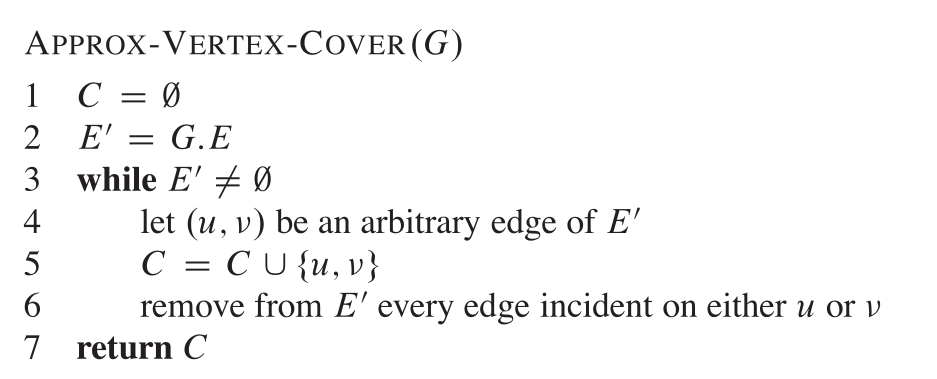
\includegraphics[scale=0.45]{figur/approxvertexcover.png}
		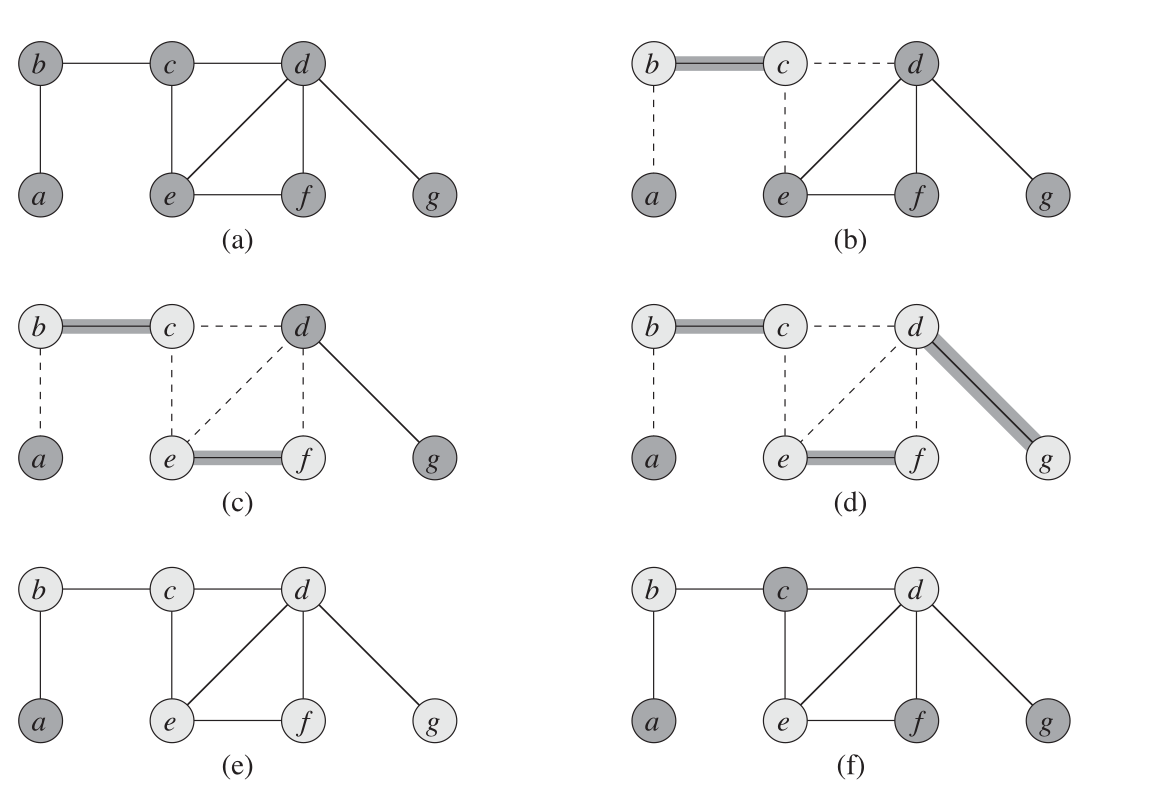
\includegraphics[scale=0.35]{figur/figur3501.png}
	\end{center}
	\begin{itemize}
		\item Køretiden af denne algoritme er $O(V+E)$, hvor vi bruger en adjacency list til at repræsentere $E'$.
	\end{itemize}

	\begin{theorem}
		\texttt{Approx-Vertex-Cover} er en polynomiel tids $2$-approksimationsalgoritme.
	\end{theorem}
	\begin{itemize}
		\item \textbf{Polynomiel tid:}
		      \begin{itemize}
			      \item Linje 1: Initialiserer $C$ til at være den tomme mængde: $O(1)$
			      \item Linje 2: Lader $E'$ være en kopi af mængden $E \in G$: $O(1)$
			      \item Linjer 3-6: Vælger en kant $(u,v) \in E'$, tilføjer $u$ og $v$ til $C$, og sletter alle kanter i $E'$ som coveres af enten $u$ eller $v$: $O(V+E)$
			      \item Linje 7: Returnerer vertex coveret $C$: $O(1)$
		      \end{itemize}

		\item Mængden $C$ af knuder der er returneret af AVC (Approx-Vertex-Cover) er et vertex cover, fordi algoritmen looper indtil alle kanter er i $C$.
		\item For at se at det er en $2$-approksimationsalgoritme:
		\item Lad $A$ være mængden af kanter som linje 4 i AVC valgte.
		\item For at cover kantene i $A$, skal ethvert vertex cover, specifikt det optimale, $C^{*}$ inkludere mindst én endpoint af hver kant i $A$.
		\item Der er ikke to kanter i $A$ som deler en endpoint, siden alle kanter der deler endpoint fjernes i linje 6.
		\item Dermed er der ikke to kanter i $A$ som er covered af den samme knude fra $C^{*}$, og dermed har vi en nedre grænse:
	\end{itemize}
	\begin{equation}
		|C^{*}| \ge |A|
	\end{equation}
	\begin{itemize}
		\item Da linje $4$ vælger en kant hvor ingen af endpointsne allerede er i $C$, har vi et upper bound på størrelsen af vertex coveret vi får af AVC:
	\end{itemize}
	\begin{equation}
		|C| = 2|A|
	\end{equation}
	\begin{itemize}
		\item Tallet $2|A|$ kommer fra de to knuder fra hver kant vi har udvalgt.
		\item Når vi kombinerer ligningerne får vi følgende:
	\end{itemize}
	\begin{align*}
		|C| & = 2|A|       \\
		    & \le 2|C^{*}|
	\end{align*}
	\begin{itemize}
		\item Som beviser sætningen.
		\item (Jeg har selv lidt brug for overbevisning her, jeg synes ikke Cormen's er specielt god.)
	\end{itemize}
\end{frame}

\begin{frame}[allowframebreaks]
	\frametitle{Traveling-salesman Problemet}
	\begin{itemize}
		\item Ved TSP (Traveling-salesman problemet) får vi tildelt en urettet graf $G = (V,E)$.
		\item $\forall (u,v) \in E : c(u,v) \ge 0$: Hver kant har et heltals ``kostefunktion''.
		\item Målet med TSP er at finde en hamiloniansk kreds af $G$ med minimums kost.
		\item Lad $c(A)$ være den totale kost af kanter i delmængden $A \subseteq E$.
	\end{itemize}

	\begin{equation*}
		c(A) = \sum_{(u,v) \in A} c(u,v)
	\end{equation*}
	\begin{itemize}
		\item I mange praktiske situationer er den billigste vej fra $u$ til $v$ at gå direkte.
		\item Vi formaliserer denne og siger at kostefunktionen $c$ satisfier trekantsuligheden (triangle inequality) hvis, $\forall u,v, w \in V$ gælder følgende:
	\end{itemize}
	\begin{equation*}
		c(u,w) \le c(u,v) + c(v,w)
	\end{equation*}
	\begin{itemize}
		\item Vi vil starte med at vise en poly-tids 2-approksimationsalgoritme til TSP med trekantsuligheden.
		\item Efter dette vil vi se at en konstant approksimationsalgoritme til TSP ikke er muligt uden trekantsuligheden undtagen hvis $P = NP$.
	\end{itemize}
\end{frame}

\begin{frame}[allowframebreaks]
	\frametitle{TSP med Trekantsulighed}
	\begin{itemize}

		\item Vi laver først et minimum spanning tree hvis vægt giver en lower bound på længden af en optimal traveling-salesman tour (altså en kreds.)
		\item Derefter bruger vi MST'et til at lave en kreds hvis kost er mindre end eller lig med det dobbelte af MST'ets vægt.
	\end{itemize}
	\begin{center}
		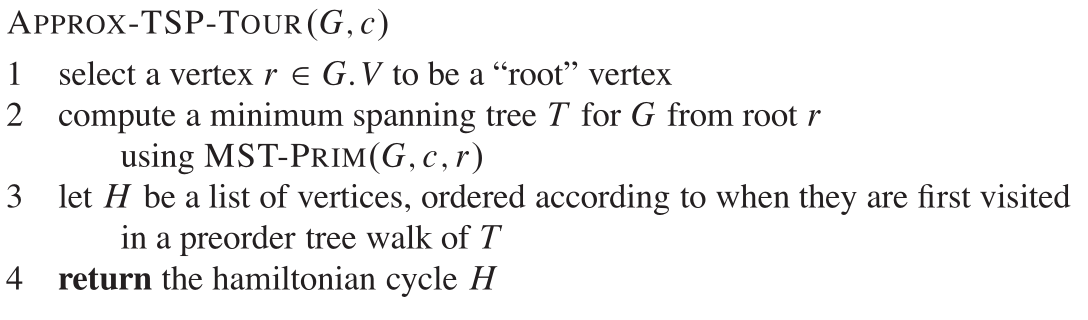
\includegraphics[scale=0.3]{figur/approxtsptour.png}
	\end{center}
	\begin{itemize}
		\item Husk her at en preorder tree walk fungerer som følger (prioriteret):
		      \begin{enumerate}
			      \item Besøg en knude
			      \item Gå til venstre
			      \item Gå til højre
		      \end{enumerate}
		\item Altså vil den gå til venstre indtil den ikke kan længere.
		\item Når den er gået til venstre går den en tilbage, og går til højre (hvis muligt.)
		\item Dette bliver den ved med indtil alle er gået igennem.
	\end{itemize}
	\begin{center}
		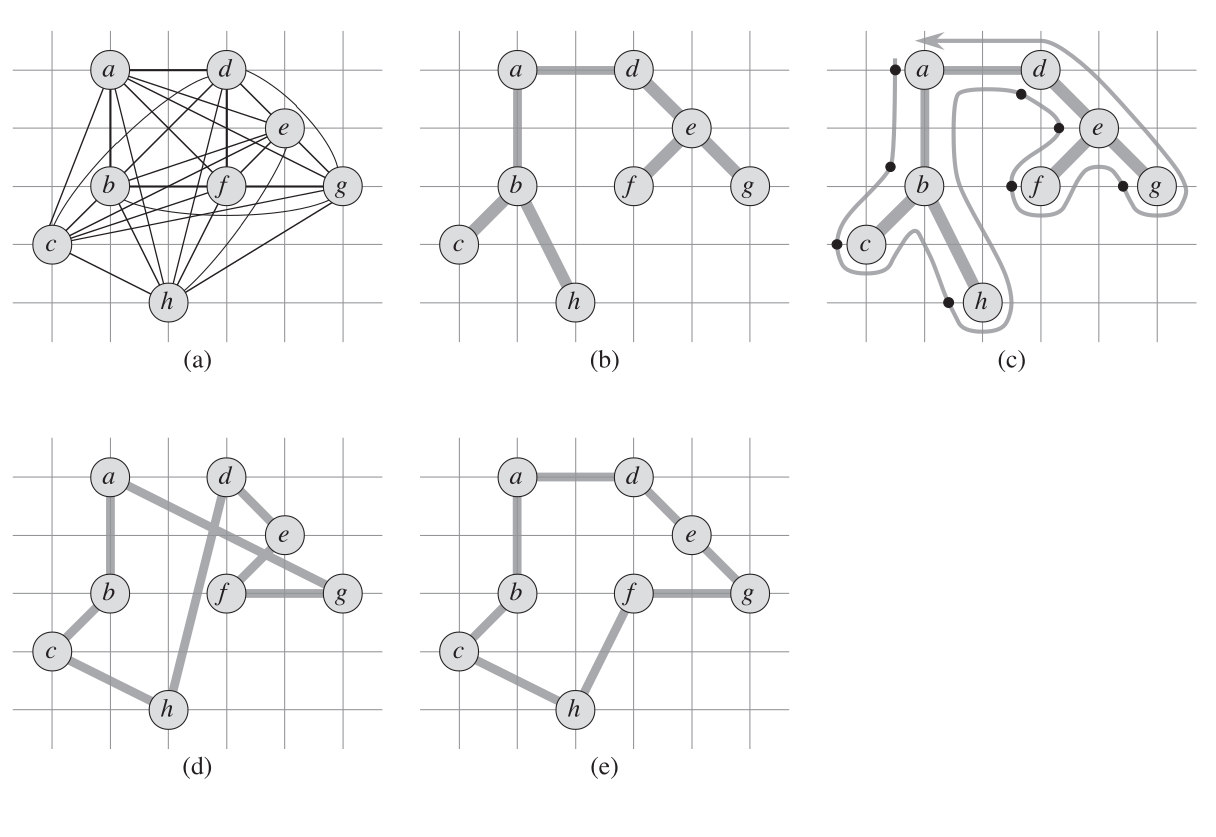
\includegraphics[scale=0.3]{figur/figur3502.png}
	\end{center}
	\begin{itemize}
		\item I figuren over, ses (d) som resultatet for algoritmen og (e) som værende den optimale kreds.
		\item Ifølge bogen (jeg ved ikke hvor tallene er fra) så har (d) en kost på ca. 19.074 og (e) har en kost på ca. 14.715.
		\item Køretiden på \textit{approx-tsp-tour} er $\Theta(V^{2})$.
		\item Bogen beskriver ikke hvorfor, og ved hjælp fra ChatGPT får jeg det til at være $\Theta(E \log V)$.
	\end{itemize}

	\begin{theorem}
		\textit{Approx-TSP-Tour} er en polynomiel-tids 2-approksimations algoritme for TSP med trekantsulighed.
	\end{theorem}

	\begin{itemize}
		\item Uanset om GPT eller bogen har ret, har vi vist at ATT kører i poly-tid.
		\item Lad $H^{*}$ være den optimale kreds, givet en mængde af knuder.
		\item Igen forklarer bogen der her forfærdeligt, men MST'et fjerner kanter, som alle har en nonnegativ værdi, og dermed får vi en lower bound på kosten af en optimal kreds:
	\end{itemize}
	\begin{equation*}
		c(T) \le c(H^{*})
	\end{equation*}

	\begin{itemize}
		\item En ``full walk'' er en liste af alle knuder når de først besøges og når end de besøges efter.
		\item Vi kalder denne fulle walk $W$, som i eksempler er:
	\end{itemize}
	\begin{equation}
		a, b, c, b, h, b , a, d, e, f, e, g, e, d, a
	\end{equation}
	\begin{itemize}
		\item Siden den fulde walk går igennem hver kant af $T$ præcis 2 gange, gælder det at:
	\end{itemize}
	\begin{equation}
		c(W) = 2c(T)
	\end{equation}
	\begin{itemize}
		\item Og ud fra den tidligere ulighed indebærer det at:
	\end{itemize}
	\begin{equation}
		c(w) \le 2c(H^{*})
	\end{equation}
	\begin{itemize}
		\item Så kosten af $W$ er altså indenfor en faktor af $2$ af kosten af en optimal kreds.
		\item Dog er $W$ ikke en kreds, fordi den går igennem knuder mere end én gang.
		\item Gennem trekantsuligheden kan vi slette et besøg til en knude fra $W$ uden at kosten bliver større.
		\item Dermed sletter vi alle knuder undtagen første gang de kommer i walken.
		\item Dermed får vi orderingen:
	\end{itemize}
	\begin{equation*}
		a, b, c, h, d, e, f, g
	\end{equation*}
	\begin{itemize}
		\item Sidne $H$ kommer far at slette knuder, får vi:
	\end{itemize}
	\begin{equation}
		c(H) \le c(W)
	\end{equation}

	\begin{itemize}
		\item Ydermere ved at kombinere denne, og $c(W) \le 2c(H^{*})$ får vi:
	\end{itemize}
	\begin{equation}
		c(H) \le 2c(H^{*})
	\end{equation}
\end{frame}

\begin{frame}[allowframebreaks]
	\frametitle{Det Generelle TSP}
	\begin{theorem}
		Hvis $P \ne NP$, så for enhver konstant \(\rho \ge 1\), eksisterer der ingen polynomiel-tids approksimationsalgoritme med et approksimationsforhold \(\rho\) for det generelle TSP.
	\end{theorem}
	\begin{itemize}
		\item Vi beviser ved modstrid.
		\item Antag at for et tal \(\rho \ge 1\), eksisterer der en polytids approksimationsalgoritme $A$, med et approksimationsforhold \(\rho\).
		\item Vi kan antage at \(\rho\) er et heltal, ved at runde op hvis nødvendigt.
		\item Vi viser nu hvordan man kan bruge $A$ til at løse instanser af hamiltoniansk kreds problemet i polynomiel tid.
		\item Lad $G = (V,E)$ være en instans a hamiltoniansk kreds problemet.
		\item Vi laver $G$ til en instans af TSP problemet som følger:

		\item Lad $G' = (V, E')$ være ne komplet graf på $V$:
		      \begin{equation}
			      E' = \{(u,v) : u, v \in V \text{ og } u \ne v\}
		      \end{equation}

		\item Vi giver en heltalskost til hver kant i $E'$ som følger:
		      \begin{equation*}
			      c(u,v) =
			      \begin{cases}
				      1           & \text{ hvis } (u,v) \in E \\
				      \rho |V| +1 & \text{ ellers}            \\
			      \end{cases}
		      \end{equation*}

		\item VI kan lave repræsentationer af $G'$ og $c$ fra en repræsentation af $G$ i polynomiel tid på $|V|$ og $|E|$.
		\item Overvej nu en instans af TSP $(G', c)$.
		\item Hvis den originale graf $G$ har en hamiltoniansk kreds $H$, så tildeler kostefunktionen $c$ til hver kant af $H$ en kost af 41, og dermed har $(G', c)$ en kreds af kost $|V|$
		\item Hvis $G$ \textbf{ikke} indeholder en hamiltoniansk kreds, så skal alle kredse af $G'$ bruge en kant der ikke er en del af $E$.
		\item Men en kreds som bruger en kant der ikke er en del af $E$ har kost:
	\end{itemize}
	\begin{align}
		(\rho|V| +1) + (|V|-1) & = \rho|V|+|V|
		                       & > \rho|V|
	\end{align}
	\begin{itemize}
		\item Fordi $A$ er garanteret til at returnere en kreds af kost ikke mere end $\rho$ ganget med kosten af en optimal tur, hvis $G$ har en hamiltoniansk kreds, så skal $A$ returnere denne.
		\item Hvis $G$ i \textbf{ikke} har en hamiltoniansk kreds, så returnerer $A$ en kreds af kosten som er mere end \(\rho|V|\).
		\item Derfor kan vi bruge $A$ til at løse hamiltoniansk-kreds problemet i polynomiel tid.
	\end{itemize}
\end{frame}

\begin{frame}[allowframebreaks]
	\frametitle{Set-Covering Problemet}
	\begin{itemize}
		\item Set-cover problemet er et optimeringsproblem, hvis decision version generaliserer vertex-cover problemet
		\item Denne algoritme har en logaritmisk approksimationsfaktor.
		\item Det vil sige, at når størrelsen af instansen bliver større, så bliver løsningen også i forhold til den optimale løsning.
		\item Logaritmefunktionen gror dog langsomt, så derfor kan denne være værd at kigge på alligevel.
		\item En instans, $(X, \mathcal{F})$ af set-covering problemet ineholder en endelig mængde $X$ og en familie $\mathcal{F}$ af delmængder af $X$, således at hvert element i $X$ er en del af mindst én delmængde i $\mathcal{F}$
		      \begin{equation*}
			      X = \bigcup_{S \in \mathcal{F}} S
		      \end{equation*}
		\item Vi siger at en delmængde $S \in F$ ``cover'' sine elementer.
		\item Problemet er at finde en minimumsstørrelse delmængde $\mathcal{C} \subseteq \mathcal{F}$, hvis medlemmer ``cover'' hele $X$:
		      \begin{equation*}
			      X = \bigcup_{S \in \mathcal{C}} S
		      \end{equation*}
	\end{itemize}
\end{frame}



%%% Local Variables:
%%% mode: latex
%%% TeX-engine: xetex
%%% TeX-command-extra-options: "-shell-escape"
%%% TeX-master: "main"
%%% End:
